\documentclass{anstrans}
%%%%%%%%%%%%%%%%%%%%%%%%%%%%%%%%%%%
\title{Pyre: A Cyclus Pyroprocessing Facility Archetype}
\author{Gregory T. Westphal and Kathryn D. Huff}

\institute{
Dept. of Nuclear, Plasma and Radiological Engineering, University of Illinois at Urbana-Champaign \\
gtw2@illinois.edu
}

%%%% packages and definitions (optional)
\usepackage{float}
\floatstyle{plaintop}
\restylefloat{table}
\usepackage{graphicx} % allows inclusion of graphics
\usepackage{booktabs} % nice rules (thick lines) for tables
\usepackage{microtype} % improves typography for PDF
\usepackage{xspace}
\usepackage{tabularx}
\newcommand{\SN}{S$_N$}
\renewcommand{\vec}[1]{\bm{#1}} %vector is bold italic
\newcommand{\vd}{\bm{\cdot}} % slightly bold vector dot
\newcommand{\grad}{\vec{\nabla}} % gradient
\newcommand{\ud}{\mathop{}\!\mathrm{d}} % upright derivative symbol
\newcommand{\Cyclus}{\textsc{Cyclus}\xspace}%
\newcommand{\Cycamore}{\textsc{Cycamore}\xspace}%
\newcolumntype{c}{>{\hsize=.56\hsize}X}
\newcolumntype{b}{>{\hsize=.7\hsize}X}
\newcolumntype{s}{>{\hsize=.74\hsize}X}
\newcolumntype{f}{>{\hsize=.1\hsize}X}
\newcolumntype{a}{>{\hsize=.45\hsize}X}

\begin{document}
%%%%%%%%%%%%%%%%%%%%%%%%%%%%%%%%%%%%%%%%%%%%%%%%%%%%%%%%%%%%%%%%%%%%%%%%%%%%%%%%
\begin{abstract}
Quantifying potential signatures and observables of material diverted from a 
pyroprocessing facility presents a modeling challenge.
This work assesses system parameters that influence separation efficiency and 
throughput. We leverage these parameters to implement a customizable pyroprocessing facility archetype for use with the Cyclus framework.
This generic facility model will allow simulations to 
quantify signatures and observables associated with various operational modes 
and material throughputs for a variety of facility designs. Such quantification 
can timely detection of material diversion. 
This paper describes the Pyre facility archetype design, pyroprocessing flowsheets captured by the model, and simulation capabilities it enables. 
To analyze data retrieved from the model, we propose a class for tracking and 
observing signatures and observables which will be extensible for other 
facility archetypes in the future.
\end{abstract}
\section{Introduction}
The diversion of significant quantities of special nuclear material from the nuclear fuel cycle is major non-proliferation 
concern \cite{noauthor_iaea_2017}. These diversions must be detected in a timely manner using signatures and observables in 
order to properly safegaurd the fuel cycle. Pyroprocessing is a used nuclear fuel separations technology capable of both 
converting current generation waste into sodium fast reactor fuel, and reprocessing next generation molten salt fuel types. 
With a new reprocessing technology comes new signatures and observables which in turn necessitate new diversion detection methods. 
The goal of this research is to identify potential signs of material diversion in a pyroprocessing facility and implement models 
of these processes into a detailed pyroprocessing facility archetype to the modular, agent-based, fuel cycle simulator, \Cyclus \cite{huff_fundamental_2016}. This facility archetype will equip users of the \Cyclus fuel cycle simulator to investigate the 
detection timeliness enabled by quantifying signatures and observables in various fuel cycle scenarios.
%%%%%%%%%%%%%%%%%%%%%%%%%%%%%%%%%%%%%%%%%%%%%%%%%%%%%%%%%%%%%%%%%%%%%%%%%%%%%%%%
\section{Background: \Cyclus}
\Cyclus models the flow of material through user-defined nuclear fuel cycle scenarios. Facilities in nuclear fuel cycles vary, 
requiring a diverse collection of pre-designed facility process models, known as \emph{archetypes}. \Cycamore, the CYClus 
Additional MOdules REpository, provides common facility archetypes (separations, enrichment, reactor, etc.)
\cite{huff_extensions_2014}. Archetypes provide a mold for users to input values specific to each facility with a known output 
\Cyclus can interpret. Simulations run in discrete time steps that allow exact isotopes to be dynamically tracked between facilities \cite{huff_fundamental_2016}. Tracking requires a form of signature or observable to follow the material accurately throughout 
and between facilities. Potentially trackable signatures and observables include truck deliveries, power draw, and steam production  \cite{Hou_2016,Yilmaz_2016}.
\Cyclus' discrete time allows users to investigate diversion and flag the time and location diversion occurs.

%%%%%%%%%%%%%%%%%%%%%%%%%%%%%%%%%%%%%%%%%%%%%%%%%%%%%%%%%%%%%%%%%%%%%%%%%%%%%%%%
\section{Background: Pyroprocessing}
Pyroprocessing is an eletrochemical separation process used to recycle spent fuel into . With the capability of processing 
various forms of waste, efficiencies will differ according to design. There are four major systems within pyroprocessing 
with observable waste: voloxidation, electroreduction, electrorefining, and electrowinning \cite{Borrelli_2017}.  

\begin{figure}[ht] % replace 't' with 'b' to force it to be on the bottom
	\centering
	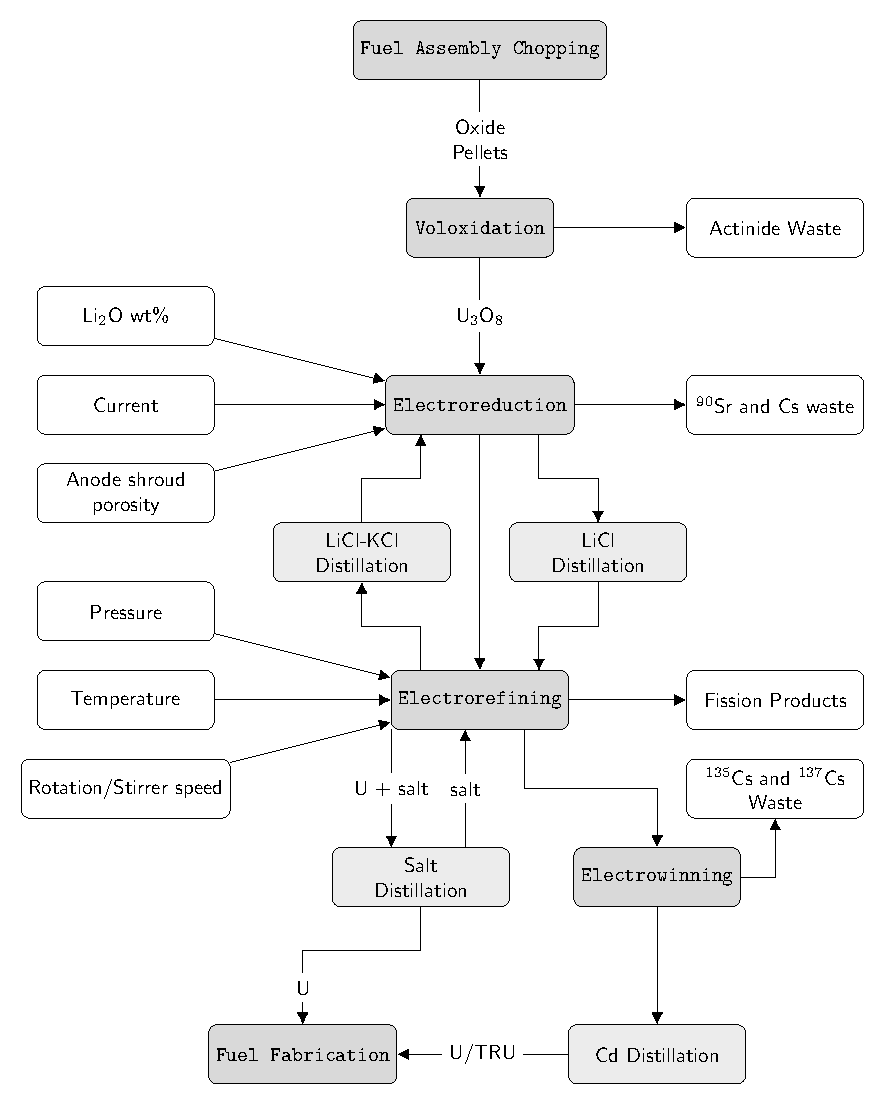
\includegraphics[width=0.5\textwidth]{flowchart}
	\caption{An archetype design flowchart of pyroprocessing facilities including observable outputs and \Cyclus variables.}
	\label{fig:flowchart}
\end{figure}

Figure 1 demonstrates the primary separations steps involved in a general pyroprocessing facility. The main process 
parameters along the left side of the flowsheet, each applied to processes most significantly impacted. The boxes on the 
right side of the processes contain the observable waste produced by each step that \Cyclus can track. Each of main processes 
are described below regarding information to be used by \Cyclus.

\subsection{Voloxidation}

For LWR fuel, the fuel must be initially treated and separated before proceeding with electrolytic processes. Heated under 
500$^{\circ}$C, noble gases and tritium are collected to decay in storage, and uranium dioxide is converted to $U_3O_8$. 
Actinides are also converted to their stable oxide forms and a majority are removed \cite{flowsheet_1998}. 

\subsection{Electroreduction}

Oxide pellets, created in voloxidation, enter the cathode, a negatively charged metal basket. Voltage between 100 and 500 mA/cm$^2$ is applied 
to the anode in a molten LiCl salt. The electrolytic reduction process primarily results in the diffusion of Cs, Ba and Sr, 
along with the reduction and conversion of zirconium into metallic form \cite{choi_electrochemical_2015,flowsheet_1998}.

\subsection{Electrorefining}

Recoverable waste from reduction is fed into an anode basket suspended in a graphite cathode. A LiCl-KCl eutectic is used as 
an electrolyte above 500$^{\circ}$C \cite{flowsheet_1998,lee_korean_2011}. The uranium dissolves at the anode to recombine at 
the cathode as metallic uranium. The waste transuranics (TRUs) and lathanides are in a soluble chloride form  while fission 
products and cladding remain in the anode basket. Finally, actinides and fission products are removed from the cladding 
electrochemically \cite{lee_korean_2011}.

\subsection{Electrowinning}

The molten salt contains TRUs from electrorefining that are separated through electrowinning with trace uranium quantities. 
With a temperature of 500$^{\circ}$C there is approximately 99 wt\% reduction in actinides and lanthanides \cite{flowsheet_1998}. 
%%%%%%%%%%%%%%%%%%%%%%%%%%%%%%%%%%%%%%%%%%%%%%%%%%%%%%%%%%%%%%%%%%%%%%%%%%%%%%%%
\section{Method: \Cyclus Simulation}
The separations facility provided by the \Cycamore library expansion is used as an initial model of a simple PRIDE facility. 
The separations archetype allows for the declaration of a feed stream and requires the user-definition of facility efficiencies. 
Each waste stream requires a material balance over voloxidation, electroreduction, electrorefining and electrowinning. The main 
waste streams are metallic waste, ceramic waste from electrowinning and electroreduction, and vitrified waste. Vitrified 
waste contains the majority of TRUs, Sr, and rare-earth elements. The elemental separation efficiencies are 
determined through theoretical material balance determined by the NEA and Hermann et al \cite{flowsheet_1998,herrmann_separation_2010}. 
The simple simulation was run to verify the table of efficiencies input to \Cyclus.

A pyroprocessing facility can be modeled with the separations archetype at low fidelity 
by a dedicated archetype. The goal for Pyre is to include facility configuration parameters and 
their respective effects on the efficiency table. Efficiencies also vary according to the feed stream resulting in different 
waste streams for LWR and FR fuels, for example. Multiple material choices exist for anodes and cathodes as well as other 
design choices that require consideration. 

\subsection{Parameters}
It's important to consider facility configuration parameters in the construction of a pyroprocessing archetype since facility designs vary in 
multiple aspects which affect the throughput and efficiencies of different waste streams. Advanced methods for electrorefining 
developed by KAERI \cite{lee_advanced_nodate} further improve salt removal efficiencies and the effect of parameter variation. 
Temperature and pressure provide a significant improvement in removal efficiency, but can vary depending on facility specifications. 

\begin{table}[h]
	\centering
	\begin{tabularx}{0.5\textwidth}{cll}
		\hline
		\textbf{Sub-process} & \textbf{Parameters} & \textbf{S \& O} \\
		\hline
		Voloxidation & Volume & Tritium \\
		& Flow Rate &  Iodine\\
		& Temperature & Technitium \\
		& Time & Actinides\\ \hline
		Electroreduction & Volume & $^{90}$Sr \\
		& Batch Size & $^{135}$Cs \\
		& Li$_2$O wt\% & $^{137}$Cs \\
		& Current & Power Draw \\
		& Porosity & Shipments \\
		& Distillation Speed & \\ \hline
		Electrorefining & Volume & Fission Products\\
		& Throughput & Power Draw \\
		& Material & Waste Salt \\
		& Anode Rotation & Vacuum Pressure\\
		& Stirrer Speed & Temperature \\
		& Pressure & \\
		& Temperature & \\ \hline
		Electrowinning & Current & Power Draw \\
		& Shroud Material & Cadmium Waste \\
		& Time & Fission Products \\
		& Flow Rate & Lanthanides \\
		&  & $^{135}$Cs \\
		&  & $^{137}$Cs \\ \hline
		Facility & Throughput & Shipments \\
		& Batch Size & Parking Lot \\
		& & Thermal Image \\
		\hline
	\end{tabularx}
	\caption {Archetype inputs and signatures \& observables at each sub-process.}
	\label {tab:pressure}
\end{table}

The data shown in Tables I and II are collected from KAERI's research into advanced electrochemical separation processes
\cite{lee_advanced_nodate}. Salt removal efficiencies mentioned are concerned with the percentage of fission products 
and salt remaining in the uranium dendrites. The evaporation coefficient represents the amount of salt evaporated due 
to vacuum pressure. As shown by Table I, the addition of vacuum pressure to the system improves removal efficiency 
with a noticeable increase between 500 and 300 mTorr. Temperature, however, exhibits the opposite effect: as temperature 
decreases so does salt removal. This comes into effect particularly depending on material choice of instrumentation and 
containment. The most limiting material choice is iron because a eutectic forms between Fe and U at 725$^{\circ}$C \cite{chapman_revision_1984}.


In facilities where iron equipment is present temperatures are limited to 700$^{\circ}$C, and efficiency is significantly 
hindered. In these advanced processes, multiple cathodes surround an agitating central anode. Cathode arrangement and anode 
rotation speed also affect the collection of uranium dendrites. Uneven, or sub-optimal, placement of cathodes result in an 
uneven electric field for electrolysis and lower efficiency while a high rotation speed causes remixing \cite{lee_advanced_nodate}. 
The addition of a central stirrer allows mixing of uranium dendrites stuck on the bottom of the vessel, improving separation 
efficiency and reducing the electroreduction time. 

Throughput is also dependent on material choice for the inert electrodes whose operating voltages vary, impacting separation 
efficiency \cite{koyama_development_2012}. A shroud surrounds the anode to provide a path for O$^{2-}$ ions to the anode and 
prevent Cl$_2$ from corroding the anode \cite{kim_development_2013,choi_electrochemical_2015}. Optimum operating current 
depends on the material choice for the anode shroud since a nonporous shroud limits ion pathways to the points of contact 
with the anode. Higher porosity corresponds to free ion paths and a higher current. With a higher current the separation 
time for reduction and winning are reduced \cite{choi_electrochemical_2015}. 


Electroreduction can further improve its throughput by the addition of Li$_2$O as a catalyst and to prevent dissolution 
of the anode \cite{choi_electrochemical_2015}. The catalyst often is used in concentration of 1 wt\% with potential for 
up to 3 wt\%. Since Li$_2$O is used to speed up the reaction, it is important to note that for signatures and observables 
the operators could add more oxide than reported to IAEA. More frequent shipments of lithium oxide can be tracked as an 
observable to match records.
%%%%%%%%%%%%%%%%%%%%%%%%%%%%%%%%%%%%%%%%%%%%%%%%%%%%%%%%%%%%%%%%%%%%%%%%%%%%%%%%
\section{Method: Proposed Algorithms}
Prior methodology explored by Hou et al. and Yilmaz et al. \cite{Hou_2016,Yilmaz_2016} consists of a minimum relative 
entropy based model and the Poisson distribution respectively. Both methods are based on similar observables for the LWR 
fuel cycle. Enrichment facilities often have set production speeds for various enrichment levels and typical shipping 
options, expedited and standard. 

\section{Discussion}
Using a material balance area over electrorefining and electroreduction yields the majority of detectable waste from 
the electrochemical processes. Electroreduction produces the majority of Sr and Cs waste with a considerable decay 
signature proportional to the efficiency and size of the feed batch \cite{Borrelli_2017,flowsheet_1998}. The electrorefining 
process also produces the fission product waste stream which requires monitoring. The following products are produced 
and tracked in this step: Tc, Ag, Pd, Rh, Ru, Mo and Zr \cite{flowsheet_1998}. Material balances over the remaining 
processes are used to verify diversion did not occur. Electrowinning produces Cs waste similar to electroreduction 
except in reduced quantities. Fuel fabrication is of high risk since finished product can be diverted with no additional 
processing steps, therefore a material balance must also be taken here. 

To determine the most significant places of diversion and where to observe them, multiple scenarios must be considered. 
Each facility parameter must be varied to observe their effects, as well as using a limited number of material balance areas. 
Scenarios will be run that include various monitoring points with the goal of determining if excess material was produced 
and what parameter was altered. For example, an increase in Cs production points to electroreduction and electrowinning. 
If both increase similarly then current is likely affected as these processes share an increase efficiency with increased 
current. Further in this scenario, if Cs production increases while Sr does not, electrowinning must be the point at which 
parameters are altered. A set of these scenarios will be used for sensitivity and importance analysis on the generic 
pyroprocessing facility.

%%%%%%%%%%%%%%%%%%%%%%%%%%%%%%%%%%%%%%%%%%%%%%%%%%%%%%%%%%%%%%%%%%%%%%%%%%%%%%%%
\section{Conclusions}
This analysis demonstrates the variability in commercialized pyroprocessing facilities and their affects on potential 
signatures and observables that will be tracked through a detailed archetype. \Cyclus also is outlined as tool in 
detecting shadow fuel cycles through its agent-based simulation and modular facilities, allowing for variations in 
plant design. Modeling and data collection of shadow fuel cycles will be performed in the \Cyclus environment after 
creation of a library specific to the unique needs of electrochemical refinement. Data from these simulations will 
be utilized in a minimum relative entropy model with additional signatures and observables to inform on detector 
placements and measurement points leading to more reliable diversion detection.

%%%%%%%%%%%%%%%%%%%%%%%%%%%%%%%%%%%%%%%%%%%%%%%%%%%%%%%%%%%%%%%%%%%%%%%%%%%%%%%%
\section{Acknowledgments}
This research was performed using funding received from the Consortium for Nonproliferation Enabling Capabilities under award number 1-483313-973000-191100.

%%%%%%%%%%%%%%%%%%%%%%%%%%%%%%%%%%%%%%%%%%%%%%%%%%%%%%%%%%%%%%%%%%%%%%%%%%%%%%%%
\bibliographystyle{ans}
\bibliography{bibliography}
\end{document}

